\documentclass[sigplan,10pt,anonymous,nonacm]{acmart}

\settopmatter{printfolios=true,printccs=false,printacmref=false}
\setcopyright{none}
\copyrightyear{2026}
\acmYear{2026}
\acmDOI{}
\acmISBN{}
\acmConference[eBPF '27]{ACM SIGCOMM Workshop on eBPF and Kernel Extensions}{2027}{TBD}

\usepackage{xspace}
\usepackage{xcolor}
\usepackage{microtype}
\setlength{\emergencystretch}{3em}
\usepackage{array}
\usepackage{tikz}
\usetikzlibrary{arrows.meta,positioning,decorations.pathreplacing}
\usepackage{listings}

\definecolor{lstkw}{HTML}{0033B3}
\definecolor{lstcmt}{HTML}{6A737D}
\definecolor{lststr}{HTML}{067D17}
\definecolor{lstnum}{HTML}{AAAAAA}
\definecolor{lsthl}{HTML}{FFF3C4}
\definecolor{lstgood}{HTML}{1B7F2E}
\definecolor{lstbad}{HTML}{C62828}

\lstdefinestyle{bpfix}{%
  basicstyle=\ttfamily\scriptsize,
  numbers=left, numberstyle=\scriptsize\color{lstnum},
  keywordstyle=\color{lstkw}\bfseries,
  commentstyle=\color{lstcmt}\itshape,
  stringstyle=\color{lststr}, showstringspaces=false,
  frame=single, framesep=3pt, rulecolor=\color{black!25},
  columns=fixed,
  breaklines=true, breakatwhitespace=true,
  numbersep=6pt,
  xleftmargin=1.5em, xrightmargin=0.5em, aboveskip=3pt, belowskip=3pt,
}

\definecolor{lstlogbg}{HTML}{EDEFF2}
\lstdefinestyle{bpflog}{%
  language=bash,
  basicstyle=\ttfamily\scriptsize,
  backgroundcolor=\color{lstlogbg},
  keywordstyle=\color{lstkw}\bfseries,
  frame=single, framesep=3pt, rulecolor=\color{black!25},
  columns=fixed,
  breaklines=true, breakatwhitespace=true,
  xleftmargin=1.5em, xrightmargin=0.5em, aboveskip=1pt, belowskip=3pt,
}

\newcommand{\zj} [1]{\textcolor{blue}{{}#1}}
\newcommand{\note} [1]{\textcolor{red}{#1}}
\newcommand{\todo} [1]{\textcolor{red}{#1}}
\newcommand{\revise} [1]{\textcolor{orange}{#1}}
\newcommand{\revised} [1]{\textcolor{green!50!gray}{#1}}

\newcommand{\sys}{\textsc{BPFOptBench}\xspace}

\newcommand{\citehere}[1][?]{%
  \textcolor{red}{[#1]}%
}


\setlength{\textfloatsep}{4pt}
\setlength{\floatsep}{4pt}
\setlength{\intextsep}{4pt}
\setlength{\abovecaptionskip}{2pt}
\setlength{\belowcaptionskip}{-3pt}

\begin{document}

\title{\sys: A Benchmark for Agentic Optimization of Existing eBPF Programs}

\author{Anonymous Authors}
\affiliation{\institution{Anonymous Institution}}
\renewcommand{\shortauthors}{Anonymous}

\begin{abstract}
Existing eBPF programs are attractive optimization targets for agents because
the action space is constrained, feedback is executable, and good decisions
require systems judgment. They are also difficult to evaluate. A candidate
rewrite must be accepted by the Linux verifier, preserve the application loader
and workload behavior, and improve the final JITed code despite noisy runtime
measurements. We propose \sys, a benchmark for agents that tune existing eBPF
programs under real verifier, JIT, and workload feedback. \sys defines frozen
optimization tasks, constrained action spaces, raw and structured feedback,
hidden evaluator checks, and component metrics for validity, workload success,
performance, regret, cost, and integrity failures. Historical corpus data
motivates the benchmark because no-op floors are large, rewrite counts do not
predict speedups, and tuned human policies improve some cases without solving
the corpus. These results argue for a benchmark and oracle first, before claiming
that current agents optimize eBPF well.
\end{abstract}

\keywords{eBPF, agents, optimization, benchmark, verifier, JIT}

\maketitle
\pagestyle{plain}

\section{Background}

eBPF lets applications extend the Linux kernel with small programs that are
loaded through application-specific control paths, checked by the in-kernel
verifier, and lowered by an architecture-specific JIT before running on events
such as packets, system calls, and profiling samples~\cite{linuxkernel-bpf-verifier,gbadamosi2024ebpf}.
Prior work shows that eBPF has real optimization and generation headroom. K2
optimizes BPF bytecode before load~\cite{xu2021synthesizing}, Merlin combines
LLVM and bytecode transformations~\cite{mao2024merlin}, and LLM-based eBPF
systems explore code generation and assistance~\cite{zheng2024kgent,simplebpf2025}.
Agent benchmarks such as SWE-bench, \(\tau\)-bench, and KernelBench show how
models can be evaluated in executable environments with hidden tests,
interaction budgets, or performance oracles~\cite{swebench2023,taubench2024,kernelbench2025}.
\sys combines these threads, but changes the unit of evaluation. The benchmark
does not ask an agent to write a fresh program or pass a verifier-only repair
task. It asks whether an agent can choose a useful optimization action for an
existing eBPF application under the real verifier/JIT/workload loop.

\section{Motivation}

Our current data supports a benchmark claim rather than an agent-performance claim.
Table~\ref{tab:motivation} summarizes the strongest evidence. The core lesson
is that verifier acceptance, rewrite applicability, JIT size, workload success,
and performance counters do not agree automatically. A benchmark that scores
only local rewrites or accepted bytecode would reward noise chasing and hide
regressions.

\begin{table}[H]
\footnotesize
\centering
\setlength{\tabcolsep}{2pt}
\caption{Existing data motivates \sys as a benchmark. Ratios are post/base unless noted.}
\label{tab:motivation}
\begin{tabular}{>{\raggedright\arraybackslash}p{0.21\linewidth}>{\raggedright\arraybackslash}p{0.34\linewidth}>{\raggedright\arraybackslash}p{0.35\linewidth}}
\hline
Evidence & Result & Benchmark implication \\
\hline
No-op floors & no-op ReJIT 0.9019 and skip-ReJIT 0.8587 over 147 programs & agents need noise gates and no-op controls \\
Pass audit & no completed standalone pass has a paper-ready improvement & rewrite count is not enough evidence \\
Full corpus & 146 programs, geomean 1.0038, 81/65 W/L & headline performance can be nearly flat \\
Applied split & changed-code rows 1.0323, unchanged rows 0.9827 & event mix and phase effects can dominate \\
Human policy & shared subset improves 0.891x to 0.898x in speedup-style reporting & choosing not to optimize is a real policy decision \\
\hline
\end{tabular}
\end{table}

\section{Design}

\sys adds a benchmark layer above an existing eBPF runner. The runner executes
real applications and records raw counters. \sys defines the task, permitted
actions, feedback surface, hidden evaluator, and scoring protocol. Each task
names a subject application, workload, architecture, baseline artifact, action
space, attempt budget, protected files, and public and hidden checks. The first
track focuses on actions that the current infrastructure can exercise, including
suite-wide pass lists, per-app policies, and per-program policies over bytecode
and live ReJIT actions. The kinsn-backed JIT capabilities are an optional
backend, not the definition of the benchmark. Source-level and LLVM-backend
actions can be added later as adapters that rebuild applications and feed the
same oracle.

\begin{figure}[H]
\centering
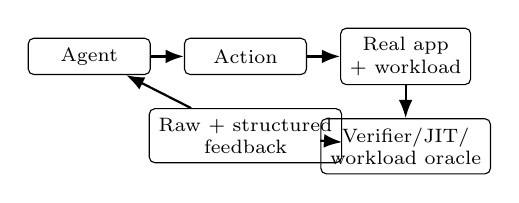
\begin{tikzpicture}[
  node distance=0.42cm,
  box/.style={draw, rounded corners=2pt, align=center, minimum width=1.55cm, minimum height=0.46cm, font=\scriptsize},
  arrow/.style={-Latex, thick}
]
\node[box] (agent) {Agent};
\node[box, right=of agent] (action) {Action};
\node[box, right=of action] (exec) {Real app\\+ workload};
\node[box, below=of exec] (oracle) {Verifier/JIT/\\workload oracle};
\node[box, below=of action] (feedback) {Raw + structured\\feedback};
\draw[arrow] (agent) -- (action);
\draw[arrow] (action) -- (exec);
\draw[arrow] (exec) -- (oracle);
\draw[arrow] (oracle) -- (feedback);
\draw[arrow] (feedback) -- (agent);
\end{tikzpicture}
\caption{\sys evaluates a closed loop in which an agent observes, chooses an
allowed optimization action, executes the real app path, and scores with a
composed oracle.}
\Description{A loop from an agent to an optimization action, real application and workload execution, verifier, JIT, and workload oracle, and raw plus structured feedback returning to the agent.}
\label{fig:loop}
\end{figure}

The oracle has hard gates before any performance score is assigned. A candidate
must be accepted by the real verifier path, preserve the application lifecycle,
pass workload-specific correctness checks, clear the task's performance
threshold or measured noise gate, and avoid forbidden shortcuts such as changing
the workload, lowering the run budget, replacing app loaders, filtering ReJIT
failures, or fabricating result files. The executor records raw artifacts only.
Ratios, geomeans, win/loss counts, confidence intervals, and scoreboards are
computed by post-hoc analysis scripts so interpretation never hides inside the
measurement path.

\section{Preliminary Evaluation}

We structure the evaluation as a benchmark-artifact study first and an
agent-performance study second. The latest v3 raw run already shows that the
execution substrate can complete the six supported macro apps
(\texttt{bcc/set}, \texttt{tracee/monitor}, \texttt{tetragon/observer},
\texttt{katran}, \texttt{cilium/agent}, and
\texttt{otelcol-ebpf-profiler/profiling}) through the native-loader path and
record per-app raw payloads. Because that run enabled no optimization passes,
it is substrate evidence rather than optimization evidence.

\begin{table}[H]
\footnotesize
\centering
\setlength{\tabcolsep}{2pt}
\caption{Preliminary evaluation plan and the claim each block can support.}
\label{tab:eval}
\begin{tabular}{>{\raggedright\arraybackslash}p{0.22\linewidth}>{\raggedright\arraybackslash}p{0.40\linewidth}>{\raggedright\arraybackslash}p{0.30\linewidth}}
\hline
Block & Method & Claim supported \\
\hline
Difficulty study & reuse no-op floors, pass audit, corpus split, and policy comparison & eBPF optimization needs a composed oracle \\
Task/evaluator audit & freeze 20--50 tasks with protected workloads and hidden checks & \sys is a reproducible benchmark artifact \\
Offline agent study & ask agents to judge signals, choose next experiments, and detect invalid actions & feedback effects can be measured \\
Small live scoreboard & compare no-op, static, random/grid, human policy, and agents on A1--A3 tasks & policies can be compared under equal budgets \\
\hline
\end{tabular}
\end{table}

The first paper should report component metrics rather than one opaque score,
including validity rate, workload success rate, performance success rate,
\texttt{bpfopt\_success\_p}, regret to the best-known valid action, attempts,
wall-clock cost, token cost, and integrity failure rate. With 20--50 audited
tasks, \sys can support a workshop benchmark claim. A stronger standalone
benchmark would require a larger public development split, a private or
rotating holdout split, and fresh-VM replay checks. The immediate goal is
therefore calibrated. We should freeze tasks and the hidden evaluator, then run
a small scoreboard that compares no-op, static, random, human-tuned, and
LLM-agent policies without claiming that current agents already solve eBPF
optimization.

\bibliographystyle{ACM-Reference-Format}
\bibliography{reference}

\end{document}
